\section{Orthogonal projections and Fourier series}

\begingroup

% definitions local to this section
\definecolor{my-yellow}{rgb}{1.00,0.87,0.00}
\definecolor{my-green}{rgb}{0,1,0}
\definecolor{my-lightblue}{rgb}{0,0.7,0.9}
\definecolor{my-blue}{rgb}{0,0,0.9}
\definecolor{my-red}{rgb}{1,0.3,0}
\definecolor{my-gray}{rgb}{0.4,0.4,0.4}

We now reconsider a problem that we briefly encountered, only in the
context of $\R^3$, in Section~\ref{sec:planes}: how to find the
shortest distance between a point and a subspace. The method we used
in Section~\ref{sec:planes} (see
Example~\ref{exa:shortest-distance-plane}) relies on the existence of
normal vectors and does not generalize beyond $\R^3$. The following
proposition gives a much better method for solving this problem,
provided that we have an orthogonal basis of the subspace.

\begin{proposition}{Orthogonal projection onto a subspace}{projection-subspace}
  Let $V$ be an inner product space, and let $W$ be a subspace of\/
  $V$. Assume $\set{\vect{u}_1,\ldots,\vect{u}_k}$ is an orthogonal
  basis of\/ $W$, and $\vect{v}\in V$ is any vector. Then the
  following vector $\vect{v}'$ is the element of $W$ that is closest
  to $\vect{v}$, i.e., such that $\norm{\vect{v}-\vect{v}'}$ is as
  small as possible.
  \begin{equation*}
    \vect{v}' =
    \frac{\iprod{\vect{u}_1,\vect{v}}}{\iprod{\vect{u}_1,\vect{u}_1}}\,\vect{u}_1
    + \frac{\iprod{\vect{u}_2,\vect{v}}}{\iprod{\vect{u}_2,\vect{u}_2}}\,\vect{u}_2
    + \ldots
    + \frac{\iprod{\vect{u}_k,\vect{v}}}{\iprod{\vect{u}_k,\vect{u}_k}}\,\vect{u}_k.
  \end{equation*}
  Moreover, the vector $\vect{v}-\vect{v}'$ is orthogonal to $W$.
  \begin{center}
    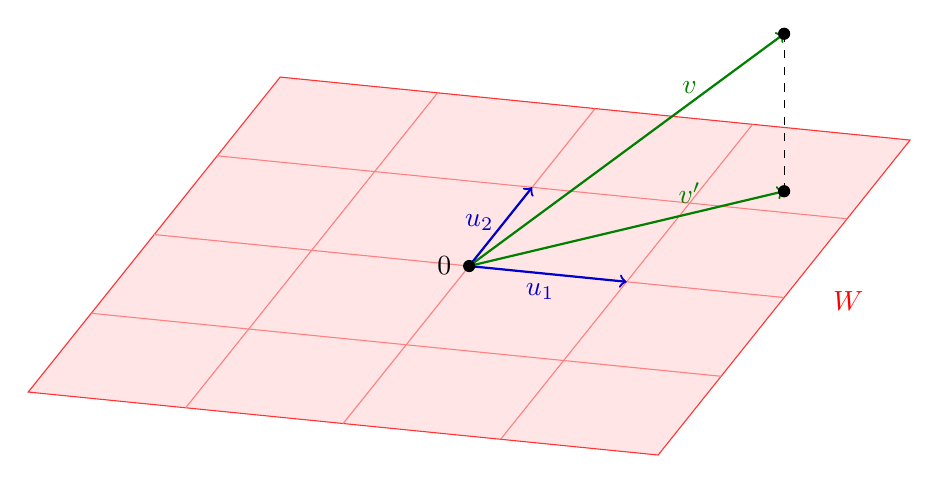
\begin{tikzpicture}[x={(1cm,-0.1cm)},y={(0.4cm,0.5cm)},z={(0cm,1cm)}]
      \filldraw[draw=red!80,fill=red!10](-4,-4,0) -- (4,-4,0) -- (4,4,0) -- (-4,4,0) -- cycle;
      \path[red] (4.5,0,0) node[right] {$W$};
      \draw[thin,red!50] (-2,-4,0) -- (-2,4,0);
      \draw[thin,red!50] (0,-4,0) -- (0,4,0);
      \draw[thin,red!50] (2,-4,0) -- (2,4,0);
      \draw[thin,red!50] (-4,-2,0) -- (4,-2,0);
      \draw[thin,red!50] (-4,0,0) -- (4,0,0);
      \draw[thin,red!50] (-4,2,0) -- (4,2,0);
      \draw[->,thick,blue!80!black](0,0,0) -- node[below, pos=0.45]{$\vect{u}_1$} (2,0,0);
      \draw[->,thick,blue!80!black](0,0,0) -- node[left, pos=0.55]{$\vect{u}_2$} (0,2,0);
      \draw[->,thick,green!50!black](0,0,0) -- node[above, pos=0.7] {$\vect{v}$} (3,2.5,2);
      \draw[->,thick,green!50!black](0,0,0) -- node[above, pos=0.7] {$\vect{v}'$} (3,2.5,0);
      \draw[dashed](3,2.5,0) -- (3,2.5,2);
      \fill (0,0,0) circle [radius=2.2pt] node [left=3pt] {$\vect{0}$};
      \fill (3,2.5,2) circle [radius=2.2pt];
      \fill (3,2.5,0) circle [radius=2.2pt];
    \end{tikzpicture}
  \end{center}
  The vector $\vect{v}'$ is called the \textbf{orthogonal projection
    of $\vect{v}$ onto $W$}%
  \index{orthogonal projection!onto subspace}%
  \index{projection!onto subspace}. We also say that $\vect{v}'$ is
  the \textbf{best approximation}%
  \index{approximation} of $\vect{v}$ in $W$.
\end{proposition}

\begin{proof}
  Since $\set{\vect{u}_1,\ldots,\vect{u}_k}$ is a basis of $W$, every
  vector $\vect{w}\in W$ is of the form
  $\vect{w} = x_1\vect{u}_1 + \ldots + x_k\vect{u}_k$, where
  $x_1,\ldots,x_k\in\R$. We have
  \begin{eqnarray*}
    \norm{\vect{v}-\vect{w}}^2
    &=& \iprod{\vect{v}-\vect{w}, \vect{v}-\vect{w}} \\
    &=& \iprod{\vect{v}, \vect{v}} - 2\iprod{\vect{w},\vect{v}} + \iprod{\vect{w},\vect{w}} \\
    &=& \iprod{\vect{v}, \vect{v}} - 2\iprod{x_1\vect{u}_1 + \ldots + x_k\vect{u}_k,\vect{v}} + \iprod{x_1\vect{u}_1 + \ldots + x_k\vect{u}_k, x_1\vect{u}_1 + \ldots + x_k\vect{u}_k} \\
    &=& \iprod{\vect{v}, \vect{v}} - 2x_1\iprod{\vect{u}_1,\vect{v}} - \ldots - 2x_k\iprod{\vect{u}_k,\vect{v}} + x_1^2\iprod{\vect{u}_1, \vect{u}_1} + \ldots + x_k^2\iprod{\vect{u}_k, \vect{u}_k} \\
    &=& \iprod{\vect{v}, \vect{v}} + (x_1^2\iprod{\vect{u}_1, \vect{u}_1} - 2x_1\iprod{\vect{u}_1,\vect{v}}) + \ldots + (x_k^2\iprod{\vect{u}_k, \vect{u}_k} - 2x_k\iprod{\vect{u}_k,\vect{v}}).
  \end{eqnarray*}
  Here, in the second-to-last step, we have used the fact that
  $\iprod{\vect{u}_i,\vect{u}_j}=0$ when $i\neq j$, i.e., the
  orthogonality of $\vect{u}_1,\ldots,\vect{u}_k$.  Therefore, the
  expression $\norm{\vect{v}-\vect{w}}^2$ is minimized when each of the
  expressions
  \begin{equation}\label{eqn:projection-subspace}
    x_1^2\iprod{\vect{u}_1, \vect{u}_1} - 2x_1\iprod{\vect{u}_1,\vect{v}}, \qquad
    \ldots,\qquad
    x_k^2\iprod{\vect{u}_k, \vect{u}_k} - 2x_k\iprod{\vect{u}_k,\vect{v}}
  \end{equation}
  takes its minimum. By the laws of calculus, the minimum of a
  function of the form $f(x)=ax^2-2bx$ occurs when $f'(x)=2ax-2b=0$,
  i.e., when $x=\frac{b}{a}$. Applying this reasoning to each of the
  $k$ expressions in {\eqref{eqn:projection-subspace}}, we find that the
  minimum occurs when
  \begin{equation*}
    x_1 = \frac{\iprod{\vect{u}_1,\vect{v}}}{\iprod{\vect{u}_1,\vect{u}_1}},\quad
    \ldots,\quad
    x_k = \frac{\iprod{\vect{u}_k,\vect{v}}}{\iprod{\vect{u}_k,\vect{u}_k}},
  \end{equation*}
  i.e., when
  \begin{equation*}
    \vect{w} =
    \frac{\iprod{\vect{u}_1,\vect{v}}}{\iprod{\vect{u}_1,\vect{u}_1}}\,\vect{u}_1
    + \frac{\iprod{\vect{u}_2,\vect{v}}}{\iprod{\vect{u}_2,\vect{u}_2}}\,\vect{u}_2
    + \ldots
    + \frac{\iprod{\vect{u}_k,\vect{v}}}{\iprod{\vect{u}_k,\vect{u}_k}}\,\vect{u}_k.
  \end{equation*}
  This is what had to be shown. Finally, to show that
  $\vect{v}-\vect{v}'$ is orthogonal to $W$, it suffices to show that
  $\vect{v}-\vect{v}'$ is orthogonal to each basis vector
  $\vect{u}_1,\ldots,\vect{u}_k$ of $W$. We show this by direct calculation.
  Consider $i\in\set{1,\ldots,k}$. First note that
  \begin{eqnarray*}
    \iprod{\vect{v}',\vect{u}_i}
    &=& \bigiprod{\paren{
        \frac{\iprod{\vect{u}_1,\vect{v}}}{\iprod{\vect{u}_1,\vect{u}_1}}\,\vect{u}_1
        + \ldots
        + \frac{\iprod{\vect{u}_k,\vect{v}}}{\iprod{\vect{u}_k,\vect{u}_k}}\,\vect{u}_k}
        ,\vect{u}_i}\\
    &=&
        \frac{\iprod{\vect{u}_1,\vect{v}}}{\iprod{\vect{u}_1,\vect{u}_1}}\,\iprod{\vect{u}_1,\vect{u}_i}
        + \ldots
        + \frac{\iprod{\vect{u}_k,\vect{v}}}{\iprod{\vect{u}_k,\vect{u}_k}}\,\iprod{\vect{u}_k,\vect{u}_i}
    \\
    &=& \frac{\iprod{\vect{u}_i,\vect{v}}}{\iprod{\vect{u}_i,\vect{u}_i}}\,\iprod{\vect{u}_i,\vect{u}_i}\\
    &=& \iprod{\vect{u}_i,\vect{v}}.
  \end{eqnarray*}
  Therefore,
  $\iprod{\vect{v}-\vect{v}',\vect{u}_i} = \iprod{\vect{v},\vect{u}_i}
  - \iprod{\vect{v}',\vect{u}_i} = 0$, and $\vect{v}-\vect{v}'$ is
  orthogonal to $\vect{u}_i$, as desired.
\end{proof}

\begin{example}{Orthogonal projection onto a subspace}{projection-subspace}
  Consider $\R^4$ with the usual dot product. Let
  $W=\sspan\set{\vect{u}_1,\vect{u}_2}$, where
  \begin{equation*}
    \vect{u}_1 = \begin{mymatrix}{r} 1 \\ 1 \\ 2 \\ 0 \end{mymatrix}, \quad
    \vect{u}_2 = \begin{mymatrix}{r} -1 \\ -1 \\ 1 \\ 3 \end{mymatrix}.
  \end{equation*}
  Note that $\vect{u}_1$ and $\vect{u}_2$ are orthogonal. Let
  \begin{equation*}
    \vect{v} = \begin{mymatrix}{r} 1 \\ 2 \\ 3 \\ 4 \end{mymatrix}.
  \end{equation*}
  Find the best approximation of $\vect{v}$ in $W$.
\end{example}

\begin{solution}
  We calculate $\iprod{\vect{u}_1,\vect{v}}=9$,
  $\iprod{\vect{u}_1,\vect{u}_1}=6$, $\iprod{\vect{u}_2,\vect{v}}=12$,
  and $\iprod{\vect{u}_2,\vect{u}_2}=12$. Therefore, by
    Proposition~\ref{prop:projection-subspace}, the desired vector is
  \begin{equation*}
    \vect{v}'
    ~=~ \frac{\iprod{\vect{u}_1,\vect{v}}}{\iprod{\vect{u}_1,\vect{u}_1}}\,\vect{u}_1
    + \frac{\iprod{\vect{u}_2,\vect{v}}}{\iprod{\vect{u}_2,\vect{u}_2}}\,\vect{u}_2
    ~=~ \frac{9}{6} \begin{mymatrix}{r} 1 \\ 1 \\ 2 \\ 0 \end{mymatrix}
    + \frac{12}{12} \begin{mymatrix}{r} -1 \\ -1 \\ 1 \\ 3 \end{mymatrix}
    ~=~ \begin{mymatrix}{c} 1/2 \\ 1/2 \\ 4 \\ 3 \end{mymatrix}.
  \end{equation*}
\end{solution}

Note how straightforward the calculations in this example are. All we
had to do is calculate a few inner products. It is not even necessary
to solve a system of equations. Such is the power of orthogonal bases.

The next example shows that we can use exactly the same method to find
approximations%
\index{approximation!of functions} of functions.

\begin{example}{Approximating a function by a polynomial}{projection-subspace-polynomial}
  Let $V=C[-1,1]$ be the vector space of continuous functions, with the
  inner product given by
  \begin{equation*}
    \iprod{f,g} = \int_{-1}^{1} f(x)g(x)\,dx.
  \end{equation*}
  Consider the function $f\in V$ given by
  \begin{equation*}
    f(x)
    ~=~ 1-\abs{x}
    ~=~ \begin{cases}
      1+x & \text{if $x<0$,} \\
      1-x & \text{if $x\geq 0$.}
    \end{cases}
  \end{equation*}
  Find the closest approximation to $f$ by a polynomial of degree at
  most 2. Graph both $f$ and the approximating polynomial.
\end{example}

\begin{solution}
  Let $W=\sspan\set{1,x,x^2}$ be the subspace of $V$ consisting of
  polynomials of degree at most 2. What we are looking for is an
  element $g\in W$ such that $\norm{f-g}$ is as small as possible.  We
  can solve this problem using
  Proposition~\ref{prop:projection-subspace}.

  First we need an orthogonal basis for $W$. We found such an
  orthogonal basis in Example~\ref{exa:legendre-polynomials}, namely
  the Legendre polynomials $p_0(x) = 1$, $p_1(x) = x$, and
  $p_2(x) = x^2-\frac{1}{3}$.  By
  Proposition~\ref{prop:projection-subspace}, the desired
  approximation $g\in W$ is given by:
  \begin{equation*}
    g
    ~=~
    \frac{\iprod{p_0,f}}{\iprod{p_0,p_0}}\,p_0
    + \frac{\iprod{p_1,f}}{\iprod{p_1,p_1}}\,p_1
    + \frac{\iprod{p_2,f}}{\iprod{p_2,p_2}}\,p_2.
  \end{equation*}
  We already computed the inner products $\iprod{p_0,p_0}=2$,
  $\iprod{p_1,p_1}=\frac{2}{3}$, and $\iprod{p_2,p_2}=\frac{8}{45}$ in
  Example~\ref{exa:legendre-polynomials}. We calculate the remaining
  inner products:
  \begin{eqnarray*}
    \iprod{p_0,f}
    &=& \int_{-1}^{1} 1\cdot f(x)\,dx
        ~=~ \int_{-1}^{0} 1\cdot (1+x)\,dx
        +   \int_{0}^{1} 1\cdot (1-x)\,dx
        ~=~ \frac{1}{2} + \frac{1}{2}
        ~=~ 1, \\
    \iprod{p_1,f}
    &=& \int_{-1}^{1} x\cdot f(x)\,\,dx
        ~=~ \int_{-1}^{0} x\cdot (1+x)\,\,dx
        +   \int_{0}^{1} x\cdot (1-x)\,\,dx
        ~=~ -\frac{1}{6} + \frac{1}{6}
        ~=~ 0, \\
    \iprod{p_2,f}
    &=& \int_{-1}^{1} (x^2-\frac{1}{3})\cdot f(x)\,dx \\
    &=& \int_{-1}^{0} (x^2-\frac{1}{3})\cdot (1+x)\,dx
        +   \int_{0}^{1} (x^2-\frac{1}{3})\cdot (1-x)\,dx
        ~=~ - \frac{1}{12} - \frac{1}{12}
        ~=~ -\frac{1}{6}.
  \end{eqnarray*}
  Therefore,
  \begin{eqnarray*}
    g
    &=&
    \frac{\iprod{p_0,f}}{\iprod{p_0,p_0}}\,p_0
        + \frac{\iprod{p_1,f}}{\iprod{p_1,p_1}}\,p_1
        + \frac{\iprod{p_2,f}}{\iprod{p_2,p_2}}\,p_2
    \\
    &=& \frac{1}{2}\,p_0
        + \frac{0}{2/3}\,p_1
        - \frac{1/6}{8/45}\,p_2
    \\
    &=& \frac{1}{2}
        - \frac{15}{16}(x^2-\frac{1}{3})
    \\
    &=& \frac{13}{16} - \frac{15}{16}x^2.
  \end{eqnarray*}
  The following graph shows the function $f(x)$ as well as the
  polynomial $g(x)$:
  \begin{center}
    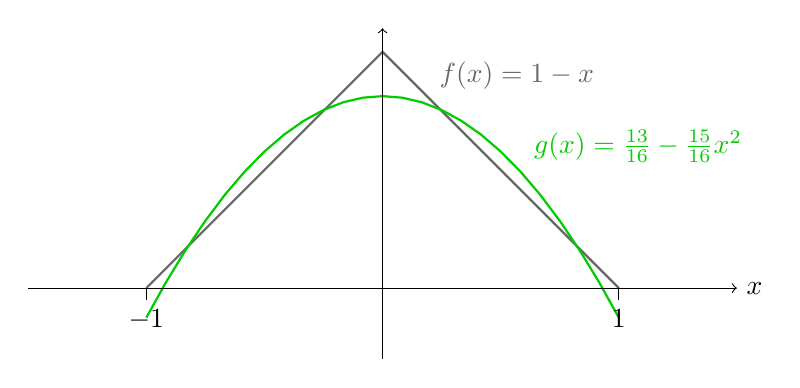
\begin{tikzpicture}[domain=-1:1, scale=3, samples=25]
      \def\fA#1{1}
      \def\fC#1{(abs((#1)^2)-1/3)}
      \draw[thick,color=my-gray] (-1,0) -- (0,1) -- (1,0);
      \draw[thick,color=my-green!80!black] plot (\x,{0.5*\fA{\x} - 0.9375*\fC{\x}});
      \path[color=my-green!80!black] (0.6,0.6) node[right]{$g(x)= \frac{13}{16} - \frac{15}{16}x^2$};
      \path[color=my-gray] (0.2,0.9) node[right]{$f(x) = 1-\abs{x}$};
      \draw[->] (-1.5,0) -- (1.5,0) node[right] {$x$};
      \draw[->] (0,-0.3) -- (0,1.1);
      \draw (1,0) -- (1,-0.05) node[below] {$1$};
      \draw (-1,0) -- (-1,-0.05) node[below] {$-1$};
    \end{tikzpicture}
  \end{center}
\end{solution}

When approximating a function $f$ by a polynomial, as in the last
example, there is no need to stop with polynomials of degree 2. We can
also ask what is the best approximation%
\index{approximation!of functions} of $f$ by a polynomial of
degree 3, of degree 4, of degree 5, and so on. By increasing the
degree of the polynomials, we get better and better approximations to
$f$. This leads us to the concept of a generalized Fourier series.

\begin{definition}{Generalized Fourier series}{generalized-fourier-series}
  Let $V$ be an inner product space and let
  $\set{\vect{u}_1,\vect{u}_2,\vect{u}_3,\ldots}$ be an infinite
  orthogonal set of vectors.  Let $\vect{v}\in V$. The
  \textbf{generalized Fourier series}%
  \index{generalized Fourier series}%
  \index{Fourier series!generalized}%
  \index{series!Fourier series} of $\vect{v}$ (with respect to
  $\vect{u}_1,\vect{u}_2,\vect{u}_3,\ldots$) consists of the following
  sequence of vectors:
  \begin{eqnarray*}
    \vect{v}_1
    &=& \frac{\iprod{\vect{u}_1,\vect{v}}}{\iprod{\vect{u}_1,\vect{u}_1}}\,\vect{u}_1, \\
    \vect{v}_2
    &=& \frac{\iprod{\vect{u}_1,\vect{v}}}{\iprod{\vect{u}_1,\vect{u}_1}}\,\vect{u}_1
        + \frac{\iprod{\vect{u}_2,\vect{v}}}{\iprod{\vect{u}_2,\vect{u}_2}}\,\vect{u}_2, \\
    \vect{v}_3
    &=& \frac{\iprod{\vect{u}_1,\vect{v}}}{\iprod{\vect{u}_1,\vect{u}_1}}\,\vect{u}_1
        + \frac{\iprod{\vect{u}_2,\vect{v}}}{\iprod{\vect{u}_2,\vect{u}_2}}\,\vect{u}_2
        + \frac{\iprod{\vect{u}_3,\vect{v}}}{\iprod{\vect{u}_3,\vect{u}_3}}\,\vect{u}_3, \\
    \vect{v}_4
    &=& \frac{\iprod{\vect{u}_1,\vect{v}}}{\iprod{\vect{u}_1,\vect{u}_1}}\,\vect{u}_1
        + \frac{\iprod{\vect{u}_2,\vect{v}}}{\iprod{\vect{u}_2,\vect{u}_2}}\,\vect{u}_2
        + \frac{\iprod{\vect{u}_3,\vect{v}}}{\iprod{\vect{u}_3,\vect{u}_3}}\,\vect{u}_3
        + \frac{\iprod{\vect{u}_4,\vect{v}}}{\iprod{\vect{u}_4,\vect{u}_4}}\,\vect{u}_4, \\
    &\vdots        &
  \end{eqnarray*}
  The vectors $\vect{v}_i$ are also called \textbf{generalized Fourier
    approximations}%
  \index{Fourier approximation}%
  \index{approximation!Fourier} of $\vect{v}$.
\end{definition}

By Proposition~\ref{prop:projection-subspace}, we know that each
$\vect{v}_i$ is the best approximation of $\vect{v}$ in the subspace
$\sspan\set{\vect{u}_1,\ldots,\vect{u}_i}$. In particular,
$\norm{\vect{v}-\vect{v}_{i+1}} \leq \norm{\vect{v}-\vect{v}_i}$, so
each $\vect{v}_i$ is potentially a better approximation of $\vect{v}$
than the previous one. In a course on analysis%
\footnote{``Algebra'' is the name for those subjects where all sums
  are finite. This includes, for example, linear algebra and abstract
  algebra. ``Analysis'' is the name for those subjects where sums are
  potentially infinite (and may or may not converge). This includes,
  for example, calculus, complex analysis, and functional analysis.},
you will learn that in many situations, the sequence
$\vect{v}_1,\vect{v}_2,\vect{v}_3,\ldots$ can be shown to converge to
$\vect{v}$.

\begin{example}{Generalized Fourier series}{generalized-fourier-series}
  Proceeding as in Example~\ref{exa:projection-subspace-polynomial},
  find the generalized Fourier approximations of $f(x)=1-\abs{x}$ up
  to degree 8.
\end{example}

\begin{solution}
  We use the Legendre polynomials $p_0,\ldots,p_8$ from
  Section~\ref{sec:gram-schmidt} and calculate the relevant inner
  products, each of which requires solving an integral. As these
  integrals get a bit complicated, it is best to use a computer
  algebra system to compute them.
  \begin{equation*}
    \def\arraystretch{1.4}
    \begin{array}{rcl}
      \iprod{p_0,f} &=& 1, \\
      \iprod{p_1,f} &=& 0, \\
      \iprod{p_2,f} &=& -\frac{1}{6}, \\
      \iprod{p_3,f} &=& 0, \\
      \iprod{p_4,f} &=& \frac{1}{105}, \\
      \iprod{p_5,f} &=& 0, \\
      \iprod{p_6,f} &=& -\frac{1}{924}, \\
      \iprod{p_7,f} &=& 0, \\
      \iprod{p_8,f} &=& \frac{1}{6435}, \\
    \end{array}
    \quad
    \begin{array}{rcl}
      \iprod{p_0,p_0} &=& 2, \\
      \iprod{p_1,p_1} &=& \frac{2}{3}, \\
      \iprod{p_2,p_2} &=& \frac{8}{45}, \\
      \iprod{p_3,p_3} &=& \frac{8}{175}, \\
      \iprod{p_4,p_4} &=& \frac{128}{11025}, \\
      \iprod{p_5,p_5} &=& \frac{128}{43659}, \\
      \iprod{p_6,p_6} &=& \frac{512}{693693}, \\
      \iprod{p_7,p_7} &=& \frac{512}{2760615}, \\
      \iprod{p_8,p_8} &=& \frac{32768}{703956825}. \\
    \end{array}
  \end{equation*}
  We therefore have the following approximations:
  \begin{eqnarray*}
    f_0 &=& f_1 ~~=~~
            \frac{1}{2}\,p_0,
    \\
    f_2 &=& f_3 ~~=~~
            \frac{1}{2}\,p_0
            - \frac{15}{16}\,p_2,
    \\
    f_4 &=& f_5 ~~=~~
            \frac{1}{2}\,p_0
            - \frac{15}{16}\,p_2
            + \frac{105}{128}\,p_4,
    \\
    f_6 &=& f_7 ~~=~~
            \frac{1}{2}\,p_0
            - \frac{15}{16}\,p_2
            + \frac{105}{128}\,p_4
            - \frac{3003}{2048}\,p_6,
    \\
    f_8 &=& f_9 ~~=~~
            \frac{1}{2}\,p_0
            - \frac{15}{16}\,p_2
            + \frac{105}{128}\,p_4
            - \frac{3003}{2048}\,p_6
            + \frac{109395}{32768}\,p_8.
  \end{eqnarray*}
  The following graph shows the function $f$ as well as its
  approximations $f_0$, $f_2$, $f_4$, $f_6$, and $f_8$. It can be seen
  that each successive approximation is closer to the function $f$
  than the previous one.
  \begin{center}
    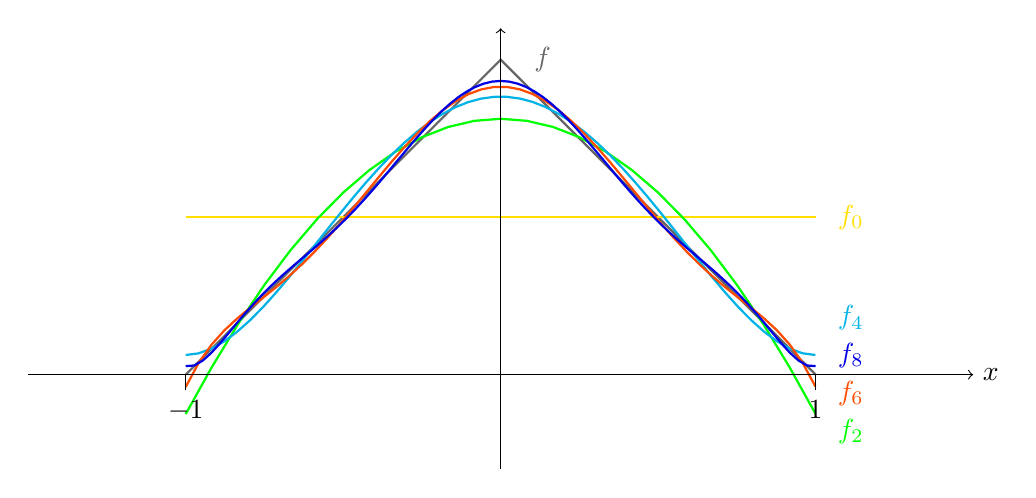
\begin{tikzpicture}[domain=-1:1, scale=4, samples=25]
      \def\fA#1{1}
      \def\fB#1{(#1)}
      \def\fC#1{(abs((#1)^2)-1/3)}
      \def\fD#1{((#1)^3-3/5*(#1))}
      \def\fE#1{(abs((#1)^4)-6/7*abs((#1)^2)+3/35)}
      \def\fF#1{((#1)^5 - 10/9*(#1)^3+5/21*(#1))}
      \def\fG#1{(abs((#1)^6)-15/11*abs((#1)^4)+5/11*abs((#1)^2)-5/231)}
      \def\fH#1{((429*(#1)^7 - 693*(#1)^5 + 315*(#1)^3 - 35*(#1))/429)}
      \def\fI#1{((6435*abs((#1)^8)-12012*abs((#1)^6)+6930*abs((#1)^4)-1260*abs((#1)^2)+35)/6435)}
      \draw[thick,color=my-gray] (-1,0) -- (0,1) -- (1,0);
      \path[color=my-gray] (0,1) node[right=2ex] {$f$};
      \draw[thick,color=my-yellow] plot (\x,0.5*\fA{\x}) (1,0.5) node[right=1ex] {$f_0$};
      \draw[thick,color=my-green] plot (\x,{0.5*\fA{\x} - 0.9375*\fC{\x}}) (1,-0.18) node[right=1ex] {$f_2$};
      \draw[thick,color=my-lightblue,samples=50] plot (\x,{0.5*\fA{\x} - 0.9375*\fC{\x} + 0.8203125*\fE{\x}}) (1,0.18) node[right=1ex] {$f_4$};
      \draw[thick,color=my-red,samples=50] plot (\x,{0.5*\fA{\x} - 0.9375*\fC{\x} + 0.8203125*\fE{\x} -1.46630859375*\fG{\x}}) (1,-0.06) node[right=1ex] {$f_6$};
      \draw[thick,color=my-blue,samples=75] plot (\x,{0.5*\fA{\x} - 0.9375*\fC{\x} + 0.8203125*\fE{\x} -1.46630859375*\fG{\x}+3.338470458984375*\fI{\x}}) (1,0.06) node[right=1ex] {$f_8$};
      \draw[->] (-1.5,0) -- (1.5,0) node[right] {$x$};
      \draw[->] (0,-0.3) -- (0,1.1);
      \draw (1,0) -- (1,-0.05) node[below] {$1$};
      \draw (-1,0) -- (-1,-0.05) node[below] {$-1$};
    \end{tikzpicture}
  \end{center}
\end{solution}

\begin{example}{Generalized Fourier series}{generalized-fourier-series2}
  The following graph shows the generalized Fourier approximations of
  the function
  \begin{equation*}
    f(x) ~=~ \begin{cases}
      0 & \mbox{if $x<0$,} \\
      1 & \mbox{if $x\geq 0$}
    \end{cases}
  \end{equation*}
  by polynomials up to degree 7. (Note: the function $f$ is not
  continuous, so not technically an element of $C[-1,1]$, but we
  ignore this here. Instead of the vector space of continuous
  functions, we can work in the vector space of piecewise continuous
  functions).
\end{example}

\begin{center}
  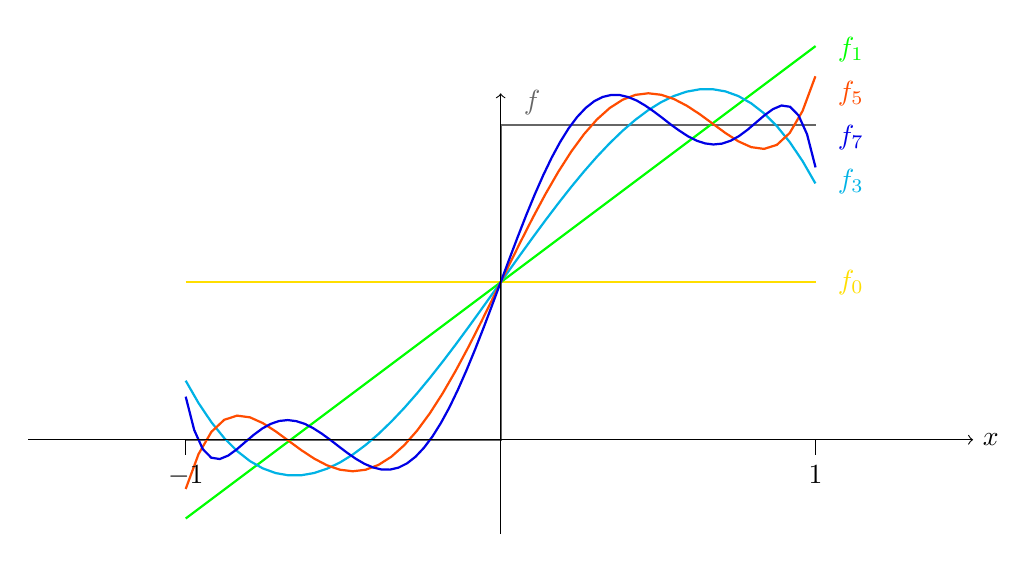
\begin{tikzpicture}[domain=-1:1, scale=4, samples=25]
    \def\fA#1{1}
    \def\fB#1{(#1)}
    \def\fC#1{(abs((#1)^2)-1/3)}
    \def\fD#1{((#1)^3-3/5*(#1))}
    \def\fE#1{(abs((#1)^4)-6/7*abs((#1)^2)+3/35)}
    \def\fF#1{((#1)^5 - 10/9*(#1)^3+5/21*(#1))}
    \def\fG#1{(abs((#1)^6)-15/11*abs((#1)^4)+5/11*abs((#1)^2)-5/231)}
    \def\fH#1{((429*(#1)^7 - 693*(#1)^5 + 315*(#1)^3 - 35*(#1))/429)}
    \def\fI#1{((6435*abs((#1)^8)-12012*abs((#1)^6)+6930*abs((#1)^4)-1260*abs((#1)^2)+35)/6435)}
    \draw[thick,color=my-gray] (-1,0) -- (0,0) -- (0,1) -- (1,1);
    \path[color=my-gray] (0.1,1) node[above] {$f$};
    \draw[thick,color=my-yellow] plot (\x,0.5*\fA{\x}) (1,0.5) node[right=1ex] {$f_0$};
    \draw[thick,color=my-green]     plot (\x,{0.5*\fA{\x} + 0.75*\fB{\x}}) (1,1.24) node[right=1ex] {$f_1$};
    \draw[thick,color=my-lightblue,samples=50]   plot (\x,{0.5*\fA{\x} + 0.75*\fB{\x} - 1.09375*\fD{\x}}) (1,0.82) node[right=1ex] {$f_3$};
    \draw[thick,color=my-red,samples=50]       plot (\x,{0.5*\fA{\x} + 0.75*\fB{\x} - 1.09375*\fD{\x} + 2.70703125*\fF{\x}}) (1,1.10) node[right=1ex] {$f_5$};
    \draw[thick,color=my-blue,samples=75]      plot (\x,{0.5*\fA{\x} + 0.75*\fB{\x} - 1.09375*\fD{\x} + 2.70703125*\fF{\x} - 7.855224609375*\fH{\x}}) (1,0.96) node[right=1ex] {$f_7$};
    \draw[->] (-1.5,0) -- (1.5,0) node[right] {$x$};
    \draw[->] (0,-0.3) -- (0,1.1);
    \draw (1,0) -- (1,-0.05) node[below] {$1$};
    \draw (-1,0) -- (-1,-0.05) node[below] {$-1$};
  \end{tikzpicture}
\end{center}

Comparing the last two examples, we see that the function in
Example~\ref{exa:generalized-fourier-series2} is much harder to
approximate well by polynomials. This is due to the discontinuity in
the latter function. Nevertheless, the sequence of approximations
eventually converges to $f$.

\begin{example}{Generalized Fourier series}{generalized-fourier-series3}
  The following graph shows the generalized Fourier approximations of
  the function
  \begin{equation*}
    f(x) ~=~ \begin{cases}
      0 & \mbox{if $x<-\frac{1}{2}$,} \\
      x+\frac{1}{2} & \mbox{if $-\frac{1}{2}\leq x<\frac{1}{2}$,} \\
      1 & \mbox{if $x\geq \frac{1}{2}$} \\
    \end{cases}
  \end{equation*}
  by polynomials up to degree 7.
\end{example}

\begin{center}
  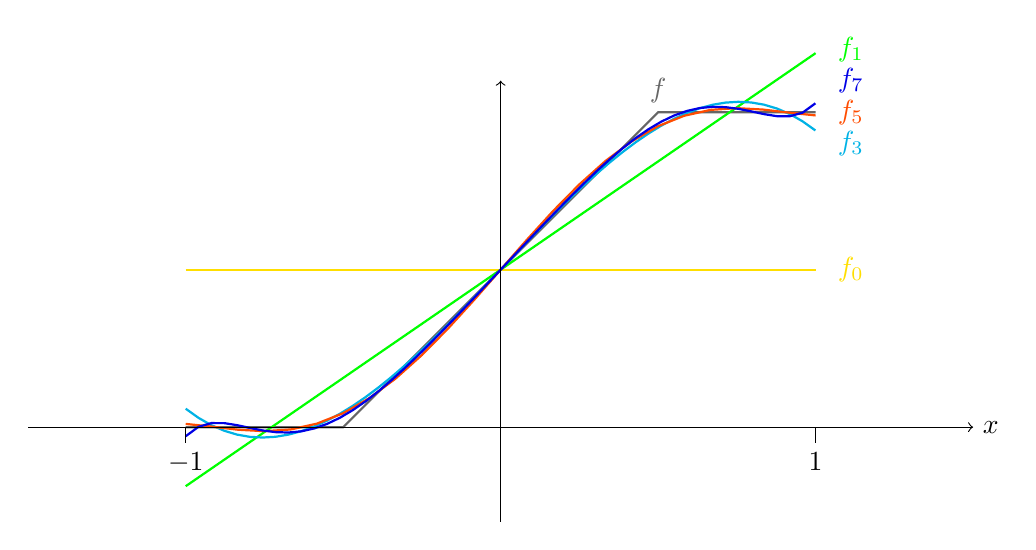
\begin{tikzpicture}[domain=-1:1, scale=4, samples=25]
    \def\fA#1{1}
    \def\fB#1{(#1)}
    \def\fC#1{(abs((#1)^2)-1/3)}
    \def\fD#1{((#1)^3-3/5*(#1))}
    \def\fE#1{(abs((#1)^4)-6/7*abs((#1)^2)+3/35)}
    \def\fF#1{((#1)^5 - 10/9*(#1)^3+5/21*(#1))}
    \def\fG#1{(abs((#1)^6)-15/11*abs((#1)^4)+5/11*abs((#1)^2)-5/231)}
    \def\fH#1{((429*(#1)^7 - 693*(#1)^5 + 315*(#1)^3 - 35*(#1))/429)}
    \def\fI#1{((6435*abs((#1)^8)-12012*abs((#1)^6)+6930*abs((#1)^4)-1260*abs((#1)^2)+35)/6435)}
    \draw[thick,color=my-gray] (-1,0) -- (-0.5,0) -- (0.5,1) -- (1,1);
    \path[color=my-gray] (0.5,1) node[above] {$f$};
    \draw[thick,color=my-yellow] plot (\x,0.5*\fA{\x}) (1,0.5) node[right=1ex] {$f_0$};
    \draw[thick,color=my-green]     plot (\x,{0.5*\fA{\x} + 0.6875*\fB{\x}}) (1,1.2) node[right=1ex] {$f_1$};
    \draw[thick,color=my-lightblue,samples=50]   plot (\x,{0.5*\fA{\x} + 0.6875*\fB{\x} - 0.615234375*\fD{\x}}) (1,0.9) node[right=1ex] {$f_3$};
    \draw[thick,color=my-red]       plot (\x,{0.5*\fA{\x} + 0.6875*\fB{\x} - 0.615234375*\fD{\x} + 0.38067626953125*\fF{\x}}) (1,1.0) node[right=1ex] {$f_5$};
    \draw[thick,color=my-blue,samples=50]      plot (\x,{0.5*\fA{\x} + 0.6875*\fB{\x} - 0.615234375*\fD{\x} + 0.38067626953125*\fF{\x} + 1.0494089126587303*\fH{\x}}) (1,1.1) node[right=1ex] {$f_7$};
    \draw[->] (-1.5,0) -- (1.5,0) node[right] {$x$};
    \draw[->] (0,-0.3) -- (0,1.1);
    \draw (1,0) -- (1,-0.05) node[below] {$1$};
    \draw (-1,0) -- (-1,-0.05) node[below] {$-1$};
  \end{tikzpicture}
\end{center}

So far, we have worked with Legendre polynomials, but there are of
course other examples of orthogonal sets of functions. An important
such set is given by sine and cosine waves. We will see that every
periodic function can be decomposed into sine and cosine waves of
varying frequencies. This was Fourier's original discovery, and the
corresponding series are just known as \textbf{Fourier series}%
\index{Fourier series}%
\index{series!Fourier series} (i.e., not ``generalized'').

\begin{example}{Fourier series}{fourier-series}
  Consider the inner product space $C[0,2\pi]$. Recall from
  Example~\ref{exa:orthogonal-set-sin-cos} that the following
  functions form an orthogonal set:
  \begin{eqnarray*}
    \vect{u}_0 &=& 1 \\
    \vect{u}_1 &=& \sin x \\
    \vect{u}_2 &=& \cos x \\
    \vect{u}_3 &=& \sin 2x \\
    \vect{u}_4 &=& \cos 2x \\
    \vect{u}_5 &=& \sin 3x \\
    \vect{u}_6 &=& \cos 3x \\
    &\vdots&
  \end{eqnarray*}
  Consider the function $f(x) = x - \pi$, where $x\in[0,2\pi]$. Find
  its Fourier series.
\end{example}

\begin{solution}
  Following Definition~\ref{def:generalized-fourier-series}, we must
  calculate a number of inner products. We have
  $\iprod{\vect{u}_0,\vect{u}_0}=2\pi$. Also, for all $i\geq 1$, we
  have $\iprod{\vect{u}_i,\vect{u}_i}=\pi$. We note the following
  antiderivatives, for $k\geq 1$:
  \begin{equation*}
    \int x\sin kx\,dx ~=~ -\frac{x}{k}\cos kx + \frac{1}{k^2}\sin kx, \qquad
    \int x\cos kx\,dx ~=~ \frac{x}{k}\sin kx + \frac{1}{k^2}\cos kx.
  \end{equation*}
  Using these formulas, we can compute the following inner products
  quite easily:
  \begin{eqnarray*}
    \iprod{\vect{u}_0, f}
    &=& \int_{0}^{2\pi} (x-\pi)
        ~~=~~ 0, \\
    \iprod{\vect{u}_1, f}
    &=& \int_{0}^{2\pi} (x-\pi)\sin x
        \,~~=~~ -2\pi, \\
    \iprod{\vect{u}_2, f}
    &=& \int_{0}^{2\pi} (x-\pi)\cos x
        ~~=~~ 0, \\
    \iprod{\vect{u}_3, f}
    &=& \int_{0}^{2\pi} (x-\pi)\sin 2x
        \,~~=~~ -\frac{2\pi}{2}, \\
    \iprod{\vect{u}_4, f}
    &=& \int_{0}^{2\pi} (x-\pi)\cos 2x
        ~~=~~ 0, \\
    \iprod{\vect{u}_5, f}
    &=& \int_{0}^{2\pi} (x-\pi)\sin 3x
        \,~~=~~ -\frac{2\pi}{3}, \\
    \iprod{\vect{u}_6, f}
    &=& \int_{0}^{2\pi} (x-\pi)\cos 3x
        ~~=~~ 0,
  \end{eqnarray*}
  and so on. We therefore find the following Fourier series:
  \begin{eqnarray*}
    f_1 &=& -2 \sin x, \\
    f_3 &=& -2 \sin x - \frac{2}{2}\sin 2x, \\
    f_5 &=& -2 \sin x - \frac{2}{2}\sin 2x - \frac{2}{3}\sin 3x, \\
    f_7 &=& -2 \sin x - \frac{2}{2}\sin 2x - \frac{2}{3}\sin 3x - \frac{2}{4}\sin 4x, \\
    f_9 &=& -2 \sin x - \frac{2}{2}\sin 2x - \frac{2}{3}\sin 3x - \frac{2}{4}\sin 4x - \frac{2}{5}\sin 5x,
  \end{eqnarray*}
  and so on. 
\end{solution}

The following graph illustrates the successive approximations of this
Fourier series.
\begin{center}
  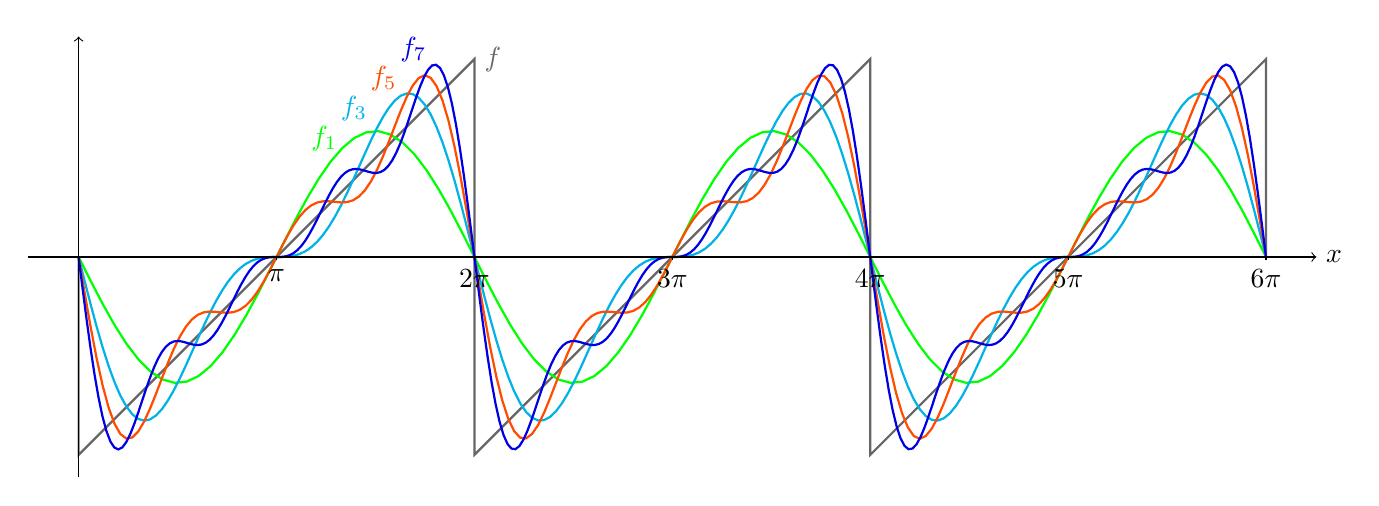
\begin{tikzpicture}[domain=0:6*pi, scale=0.8, samples=100]
    \def\fA#1{1}
    \def\fB#1{(sin((#1)/pi*180)}
    \def\fC#1{(cos((#1)/pi*180))}
    \def\fD#1{(sin(2*(#1)/pi*180))}
    \def\fE#1{(cos(2*(#1)/pi*180))}
    \def\fF#1{(sin(3*(#1)/pi*180))}
    \def\fG#1{(cos(3*(#1)/pi*180))}
    \def\fH#1{(sin(4*(#1)/pi*180))}
    \def\fI#1{(cos(4*(#1)/pi*180))}
    \draw[thick,color=my-gray] (0,0) -- (0,-pi) -- (2*pi,pi) -- (2*pi,-pi) -- (4*pi,pi) -- (4*pi,-pi) -- (6*pi, pi) -- (6*pi, 0) (2*pi, pi) node[right] {$f$};
    \draw[thick,color=my-green]                 plot (\x,{((-2)*\fB{\x})}) (pi,0) +(0.6*pi,0.6*pi) node[left=4ex] {$f_1$};
    \draw[thick,color=my-lightblue,samples=200] plot (\x,{((-2)*\fB{\x})+((-1)*\fD{\x})}) (pi,0) +(0.75*pi,0.75*pi) node[left=4ex] {$f_3$};
    \draw[thick,color=my-red,samples=200]       plot (\x,{((-2)*\fB{\x})+((-1)*\fD{\x})+((-2/3)*\fF{\x})}) (pi,0) +(0.9*pi,0.9*pi) node[left=4ex] {$f_5$};
    \draw[thick,color=my-blue,samples=300]      plot (\x,{((-2)*\fB{\x})+((-1)*\fD{\x})+((-2/3)*\fF{\x})+((-1/2)*\fH{\x})}) (pi,0) +(1.05*pi,1.05*pi) node[left=4ex] {$f_7$};
    \draw[->] (-0.8,0) -- (6*pi+0.8,0) node[right] {$x$};
    \draw[->] (0,-3.5) -- (0,3.5);
    \draw (pi,0) -- (pi,-0.05) node[below] {$\pi$};
    \draw (2*pi,0) -- (2*pi,-0.05) node[below] {$2\pi$};
    \draw (3*pi,0) -- (3*pi,-0.05) node[below] {$3\pi$};
    \draw (4*pi,0) -- (4*pi,-0.05) node[below] {$4\pi$};
    \draw (5*pi,0) -- (5*pi,-0.05) node[below] {$5\pi$};
    \draw (6*pi,0) -- (6*pi,-0.05) node[below] {$6\pi$};
  \end{tikzpicture}
\end{center}
Note that, although the function $f$ is defined on the interval
$[0,2\pi]$, we have extended it periodically for $[2\pi,4\pi]$,
$[4\pi,6\pi]$, and so on. This makes sense because all of the
orthogonal functions $1$, $\sin x$, $\cos x$, $\sin 2x$, and so on,
have period $2\pi$.

We can also illustrate the same information differently, by showing
the individual sine waves making up the wave form of the function
$f(x)$. In the context of audio signals, these sine waves are also
called the \textbf{harmonics}%
\index{harmonic} of the signal.

\begin{center}
  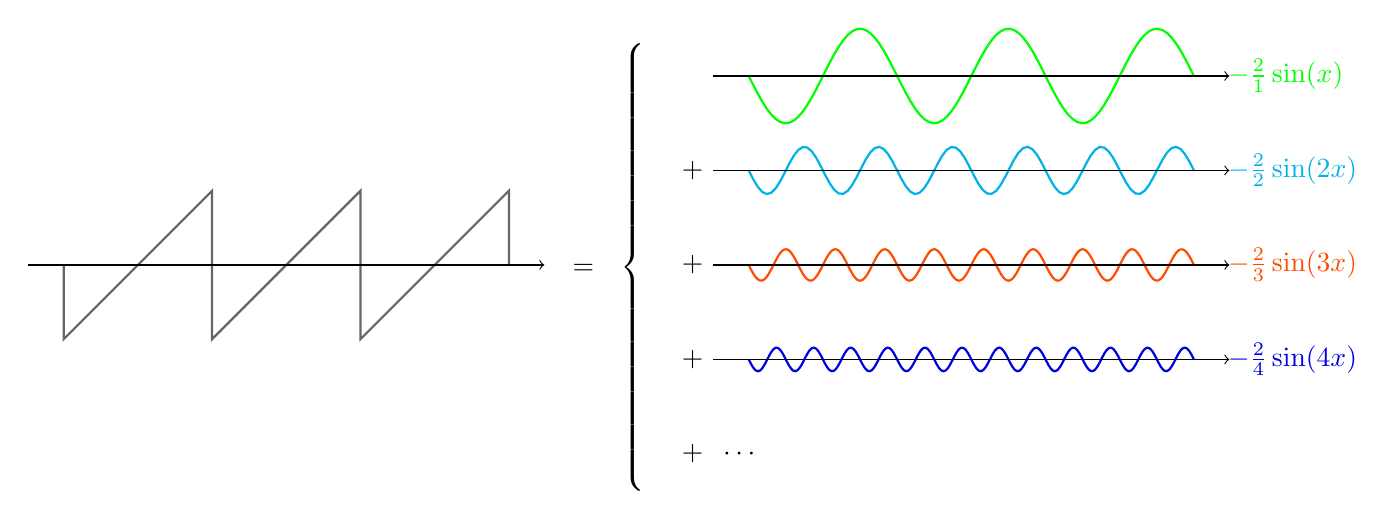
\begin{tikzpicture}[domain=0:6*pi, scale=0.3, samples=100]
    \def\fA#1{1}
    \def\fB#1{(sin((#1)/pi*180)}
    \def\fC#1{(cos((#1)/pi*180))}
    \def\fD#1{(sin(2*(#1)/pi*180))}
    \def\fE#1{(cos(2*(#1)/pi*180))}
    \def\fF#1{(sin(3*(#1)/pi*180))}
    \def\fG#1{(cos(3*(#1)/pi*180))}
    \def\fH#1{(sin(4*(#1)/pi*180))}
    \def\fI#1{(cos(4*(#1)/pi*180))}
    \begin{scope}[yshift=-12cm,xshift=-29cm]
      \draw[thick,color=my-gray] (0,0) -- (0,-pi) -- (2*pi,pi) -- (2*pi,-pi) --
      (4*pi,pi) -- (4*pi,-pi) -- (6*pi, pi) -- (6*pi, 0);
      \draw[->] (-1.5,0) -- (6*pi+1.5,0)
      node[right]{$~~=~~\left\{\rule{0mm}{3cm}\right.$};
    \end{scope}
    \begin{scope}[yshift=-4cm]
      \draw[thick,color=my-green]   plot (\x,{((-2)*\fB{\x})}) node[right=2ex] {$-\frac{2}{1}\sin(x)$};
      \draw[->] (-1.5,0) -- (6*pi+1.5,0);
    \end{scope}
    \begin{scope}[yshift=-8cm]
      \draw[thick,color=my-lightblue] plot (\x,{((-1)*\fD{\x})}) node[right=2ex] {$-\frac{2}{2}\sin(2x)$};
      \draw[->] (-1.5,0) node[left]{$+$} -- (6*pi+1.5,0);
    \end{scope}
    \begin{scope}[yshift=-12cm]
      \draw[thick,color=my-red,samples=200]     plot (\x,{((-2/3)*\fF{\x})}) node[right=2ex] {$-\frac{2}{3}\sin(3x)$};
      \draw[->] (-1.5,0) node[left]{$+$} -- (6*pi+1.5,0);
    \end{scope}
    \begin{scope}[yshift=-16cm]
      \draw[thick,color=my-blue,samples=200]    plot (\x,{((-1/2)*\fH{\x})}) node[right=2ex] {$-\frac{2}{4}\sin(4x)$};
      \draw[->] (-1.5,0) node[left]{$+$} -- (6*pi+1.5,0);
    \end{scope}
    \begin{scope}[yshift=-20cm]
      \path (-1.5,0) node[left]{$+$} node[right]{$\cdots$};
    \end{scope}
  \end{tikzpicture}
\end{center}

\begin{example}{Fourier series}{fourier-series2}
  The following graph shows the first few Fourier approximations of the function
  \begin{equation*}
    f(x) ~=~ \begin{cases}
      x - \frac{\pi}{2} & \mbox{if $0\leq x<\pi$,} \\
      \frac{3\pi}{2} - x & \mbox{if $\pi\leq x\leq 2\pi$.}
    \end{cases}
  \end{equation*}
\end{example}
      
\begin{center}
  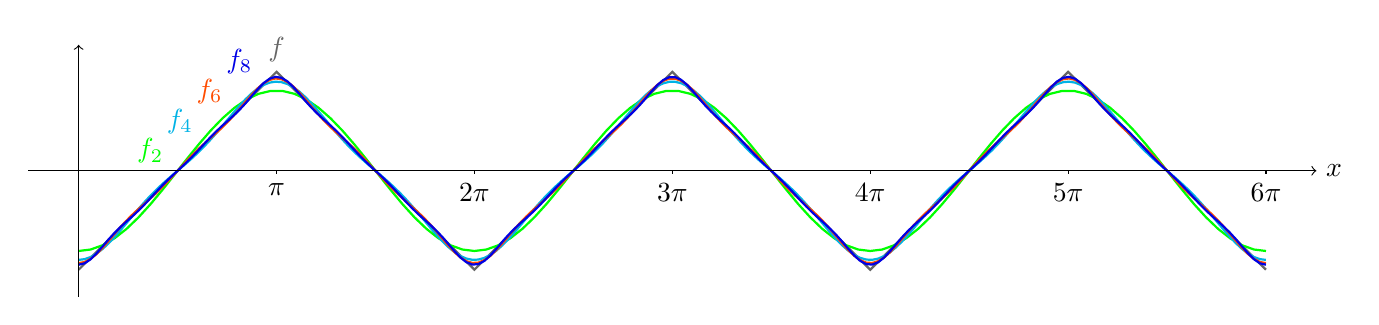
\begin{tikzpicture}[domain=0:6*pi, scale=0.8, samples=100]
    \def\fC#1{(cos((#1)/pi*180))}
    \def\fG#1{(cos(3*(#1)/pi*180))}
    \def\fK#1{(cos(5*(#1)/pi*180))}
    \def\fO#1{(cos(7*(#1)/pi*180))}
    \draw[thick,color=my-gray] (0,-pi/2) -- (pi,pi/2) -- (2*pi,-pi/2) -- (3*pi,pi/2) -- (4*pi,-pi/2) -- (5*pi,pi/2) -- (6*pi, -pi/2) (pi,pi/2) node [above] {$f$};
    \draw[thick,color=my-green]   plot (\x,{((-1.2732395447351623)*\fC{\x})}) (0.6*pi,-pi/2+0.6*pi) node[left=2ex] {$f_2$};
    \draw[thick,color=my-lightblue,samples=200] plot (\x,{((-1.2732395447351623)*\fC{\x})+((-0.14147106052612904)*\fG{\x})}) (0.75*pi,-pi/2+0.75*pi) node[left=2ex] {$f_4$};
    \draw[thick,color=my-red,samples=200]     plot (\x,{((-1.2732395447351623)*\fC{\x})+((-0.14147106052612904)*\fG{\x})+((-0.05092958178940641)*\fK{\x})}) (0.9*pi,-pi/2+0.9*pi) node[left=2ex] {$f_6$};
    \draw[thick,color=my-blue,samples=200]    plot (\x,{((-1.2732395447351623)*\fC{\x})+((-0.14147106052612904)*\fG{\x})+((-0.05092958178940641)*\fK{\x})+((-0.025984480504798825)*\fO{\x})}) (1.05*pi,-pi/2+1.05*pi) node[left=2ex] {$f_8$};
    \draw[->] (-0.8,0) -- (6*pi+0.8,0) node[right] {$x$};
    \draw[->] (0,-2) -- (0,2);
    \draw (pi,0) -- (pi,-0.05) node[below] {$\pi$};
    \draw (2*pi,0) -- (2*pi,-0.05) node[below] {$2\pi$};
    \draw (3*pi,0) -- (3*pi,-0.05) node[below] {$3\pi$};
    \draw (4*pi,0) -- (4*pi,-0.05) node[below] {$4\pi$};
    \draw (5*pi,0) -- (5*pi,-0.05) node[below] {$5\pi$};
    \draw (6*pi,0) -- (6*pi,-0.05) node[below] {$6\pi$};
  \end{tikzpicture}
\end{center}

\noindent Note how rapidly this Fourier series converges to $f$. The
following image shows the function $f$ (extended periodically outside
the interval $[0,2\pi]$) as a sum of its harmonics. Compared to
Example~\ref{exa:fourier-series}, we see that the higher harmonics
have much smaller amplitudes, which explains the rapid convergence.

\begin{center}
  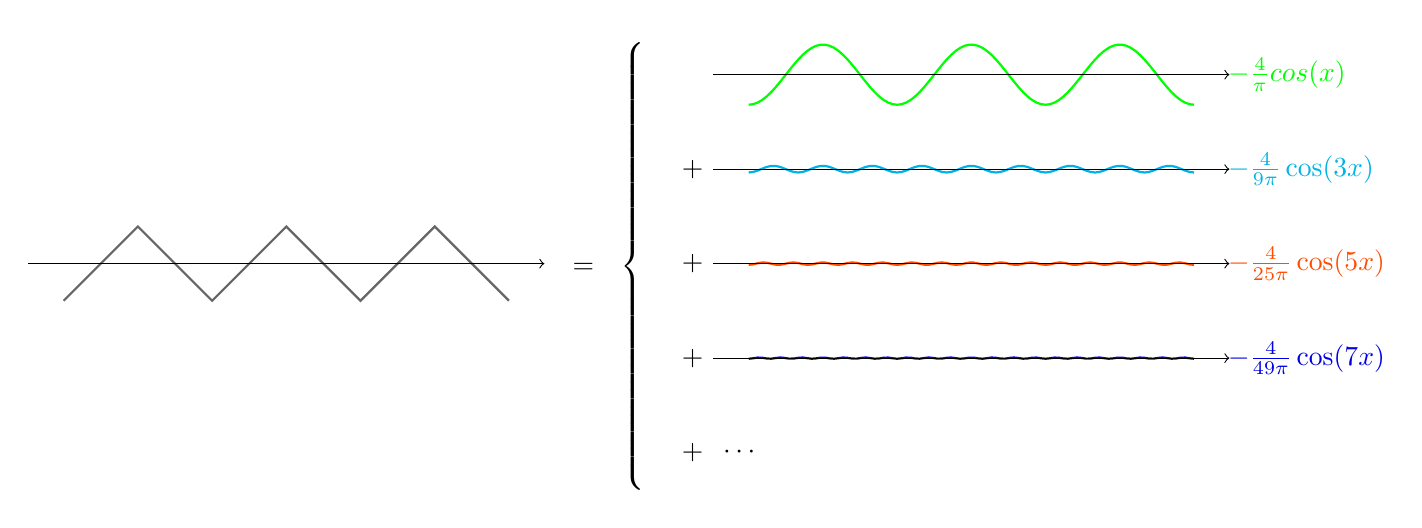
\begin{tikzpicture}[domain=0:6*pi, scale=0.3, samples=100]
    \def\fC#1{(cos((#1)/pi*180))}
    \def\fG#1{(cos(3*(#1)/pi*180))}
    \def\fK#1{(cos(5*(#1)/pi*180))}
    \def\fO#1{(cos(7*(#1)/pi*180))}
    \begin{scope}[yshift=-12cm,xshift=-29cm]
      \draw[thick,color=my-gray] (0,-pi/2) -- (pi,pi/2) -- (2*pi,-pi/2) -- (3*pi,pi/2) --
      (4*pi,-pi/2) -- (5*pi,pi/2) -- (6*pi, -pi/2);
      \draw[->] (-1.5,0) -- (6*pi+1.5,0)
      node[right]{$~~=~~\left\{\rule{0mm}{3cm}\right.$};
    \end{scope}
    \begin{scope}[yshift=-4cm]
      \draw[thick,color=my-green]   plot (\x,{((-1.2732395447351623)*\fC{\x})}) (6*pi,0) node[right=2ex] {$-\frac{4}{\pi}cos(x)$};
      \draw[->] (-1.5,0) -- (6*pi+1.5,0);
    \end{scope}
    \begin{scope}[yshift=-8cm]
      \draw[thick,color=my-lightblue] plot (\x,{((-0.14147106052612904)*\fG{\x})}) (6*pi,0) node[right=2ex] {$-\frac{4}{9\pi}\cos(3x)$};
      \draw[->] (-1.5,0) node[left]{$+$} -- (6*pi+1.5,0);
    \end{scope}
    \begin{scope}[yshift=-12cm]
      \draw[thick,color=my-red]     plot (\x,{((-0.05092958178940641)*\fK{\x})}) (6*pi,0) node[right=2ex] {$-\frac{4}{25\pi}\cos(5x)$};
      \draw[->] (-1.5,0) node[left]{$+$} -- (6*pi+1.5,0);
    \end{scope}
    \begin{scope}[yshift=-16cm]
      \draw[thick,color=my-blue]    plot (\x,{((-0.025984480504798825)*\fO{\x})}) (6*pi,0) node[right=2ex] {$-\frac{4}{49\pi}\cos(7x)$};
      \draw[->] (-1.5,0) node[left]{$+$} -- (6*pi+1.5,0);
    \end{scope}
    \begin{scope}[yshift=-20cm]
      \path (-1.5,0) node[left]{$+$} node[right]{$\cdots$};
    \end{scope}
  \end{tikzpicture}
\end{center}

\begin{example}{Fourier series}{fourier-series3}
  The following graph shows the first few Fourier approximations of the function
  \begin{equation*}
    f(x) ~=~ \begin{cases}
      1 & \mbox{if $0\leq x<\pi$,} \\
      -1 & \mbox{if $\pi\leq x\leq 2\pi$.}
    \end{cases}
  \end{equation*}
\end{example}
      
\begin{center}
  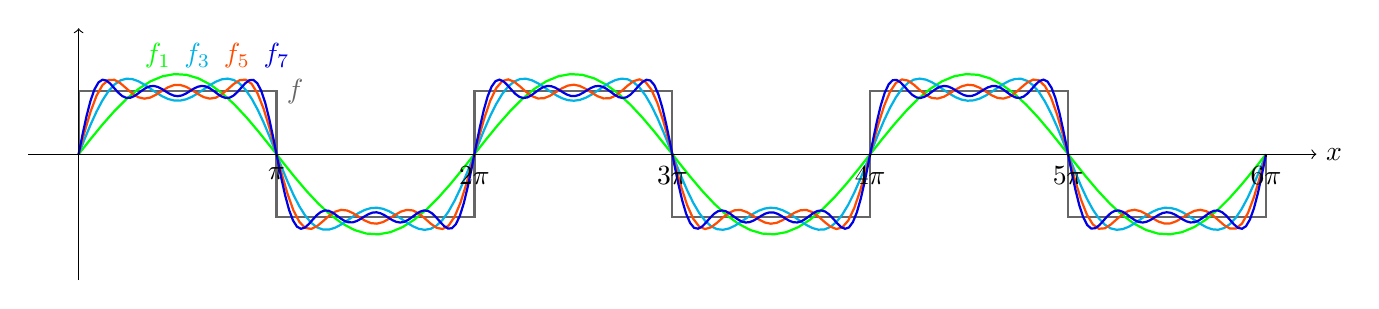
\begin{tikzpicture}[domain=0:6*pi, scale=0.8, samples=100]
    \def\fB#1{(sin((#1)/pi*180))}
    \def\fF#1{(sin(3*(#1)/pi*180))}
    \def\fJ#1{(sin(5*(#1)/pi*180))}
    \def\fN#1{(sin(7*(#1)/pi*180))}
    \draw[thick,color=my-gray] (0,0) -- (0,1) -- (pi,1) -- (pi,-1) --
    (2*pi,-1) -- (2*pi,1) --
    (3*pi,1) -- (3*pi,-1) --
    (4*pi,-1) -- (4*pi,1) --
    (5*pi,1) -- (5*pi,-1) --
    (6*pi,-1) -- (6*pi,0) (pi, 1) node[right] {$f$};
    \draw[thick,color=my-green]   plot (\x,{((1.2732395447351623)*\fB{\x})}) (0.4*pi, 1.2) node[above] {$f_1$};
    \draw[thick,color=my-lightblue,samples=200] plot (\x,{((1.2732395447351623)*\fB{\x})+((0.4244131815783881)*\fF{\x})}) (0.6*pi, 1.2) node[above] {$f_3$};
    \draw[thick,color=my-red,samples=200]     plot (\x,{((1.2732395447351623)*\fB{\x})+((0.4244131815783881)*\fF{\x})+((0.25464790894703326)*\fJ{\x})}) (0.8*pi, 1.2) node[above] {$f_5$};
    \draw[thick,color=my-blue,samples=300]    plot (\x,{((1.2732395447351623)*\fB{\x})+((0.4244131815783881)*\fF{\x})+((0.25464790894703326)*\fJ{\x})+((0.18189136353359486)*\fN{\x})}) (1.0*pi, 1.2) node[above] {$f_7$};
    \draw[->] (-0.8,0) -- (6*pi+0.8,0) node[right] {$x$};
    \draw[->] (0,-2) -- (0,2);
    \draw (pi,0) -- (pi,-0.05) node[below] {$\pi$};
    \draw (2*pi,0) -- (2*pi,-0.05) node[below] {$2\pi$};
    \draw (3*pi,0) -- (3*pi,-0.05) node[below] {$3\pi$};
    \draw (4*pi,0) -- (4*pi,-0.05) node[below] {$4\pi$};
    \draw (5*pi,0) -- (5*pi,-0.05) node[below] {$5\pi$};
    \draw (6*pi,0) -- (6*pi,-0.05) node[below] {$6\pi$};
  \end{tikzpicture}
\end{center}

\noindent Once again, here is an image showing the function $f$ as a
sum of its harmonics:

\begin{center}
  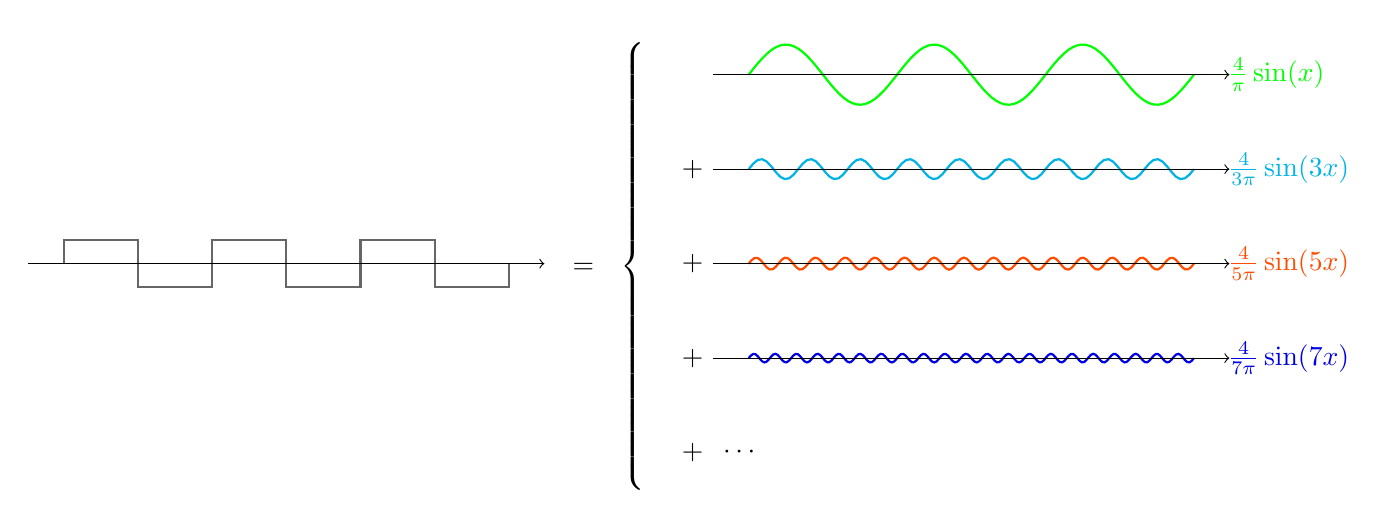
\begin{tikzpicture}[domain=0:6*pi, scale=0.3, samples=100]
    \def\fB#1{(sin((#1)/pi*180))}
    \def\fF#1{(sin(3*(#1)/pi*180))}
    \def\fJ#1{(sin(5*(#1)/pi*180))}
    \def\fN#1{(sin(7*(#1)/pi*180))}
    \begin{scope}[yshift=-12cm,xshift=-29cm]
      \draw[thick,color=my-gray] (0,0) -- (0,1) -- (pi,1) -- (pi,-1) --
      (2*pi,-1) -- (2*pi,1) --
      (3*pi,1) -- (3*pi,-1) --
      (4*pi,-1) -- (4*pi,1) --
      (5*pi,1) -- (5*pi,-1) --
      (6*pi,-1) -- (6*pi,0);
      \draw[->] (-1.5,0) -- (6*pi+1.5,0)
      node[right]{$~~=~~\left\{\rule{0mm}{3cm}\right.$};
    \end{scope}
    \begin{scope}[yshift=-4cm]
      \draw[thick,color=my-green]   plot (\x,{((1.2732395447351623)*\fB{\x})}) node[right=2ex] {$\frac{4}{\pi}\sin(x)$};
      \draw[->] (-1.5,0) -- (6*pi+1.5,0);
    \end{scope}
    \begin{scope}[yshift=-8cm]
      \draw[thick,color=my-lightblue] plot (\x,{((0.4244131815783881)*\fF{\x})}) node[right=2ex] {$\frac{4}{3\pi}\sin(3x)$};
      \draw[->] (-1.5,0) node[left]{$+$} -- (6*pi+1.5,0);
    \end{scope}
    \begin{scope}[yshift=-12cm]
      \draw[thick,color=my-red,samples=150]     plot (\x,{((0.25464790894703326)*\fJ{\x})}) node[right=2ex] {$\frac{4}{5\pi}\sin(5x)$};
      \draw[->] (-1.5,0) node[left]{$+$} -- (6*pi+1.5,0);
    \end{scope}
    \begin{scope}[yshift=-16cm]
      \draw[thick,color=my-blue,samples=200]    plot (\x,{((0.18189136353359486)*\fN{\x})}) node[right=2ex] {$\frac{4}{7\pi}\sin(7x)$};
      \draw[->] (-1.5,0) node[left]{$+$} -- (6*pi+1.5,0);
    \end{scope}
    \begin{scope}[yshift=-20cm]
      \path (-1.5,0) node[left]{$+$} node[right]{$\cdots$};
    \end{scope}
  \end{tikzpicture}
\end{center}

\noindent
Watch the video at \url{http://y2u.be/3IAMpH4xF9Q} for a demonstration
of how the functions from
Examples~\ref{exa:fourier-series}--\ref{exa:fourier-series3}, and
their harmonics, sound as audio signals.

\endgroup
